\section{Auswertung}
\subsection{Dämpfung}
Nach Gl. \ref{eqn:Absorption} beschreibt $\alpha$ den Absorbtionskoeffizenten, und
somit die Dämpfung der Intensität.
Für das Impuls-Echo-Verfahren ergibt sich für eine Länge $L$ eines Zylinders
\begin{equation}
    I(2L)=I_0e^{-\alpha 2L},
\end{equation}
mit
\begin{equation}
    \alpha=-\frac{1}{2L}\text{ln}\left(\frac{I(2L)}{I_0}\right).
\end{equation}
\begin{table}
    \centering
    \begin{tabular}{c|c c c}
        \toprule
        &Zylinder 1 &Zylinder 2&Zylinder 3\\
        \midrule
        Länge $L$ [cm] &30&40.04&120.04\\
        $I(2L)$ [V] &1.33&0.7&0.11\\
        $I_0$ [V]& 1.33&1.35&1.34\\
        $t$ [$\mu$s]&30&59.8&88.9\\
        \midrule
        $\alpha$ [cm$^{-1}$]& 0&0.004&0.01\\
        \bottomrule
    \end{tabular}
    \caption{}
    \label{tab:wertetabelle}
\end{table}

\subsection{Schallgschwindigkeitsbestimmung (Impuls-Echo)}
Die Bestimmung der Schallgeschwindikeit der Schallgeschwindigkeit der Anpassungschicht
der Sonde kann mithilfe der Laufzeit $t$ (siehe Tab. \ref{tab:wertetabelle}) erzielt werden.


Dafür wird die Laufzeit (hier nun $\frac{t}{2}$) gegen die Länge $L$ der Zylinder aufgetragen.
\begin{figure}[H]
    \centering
    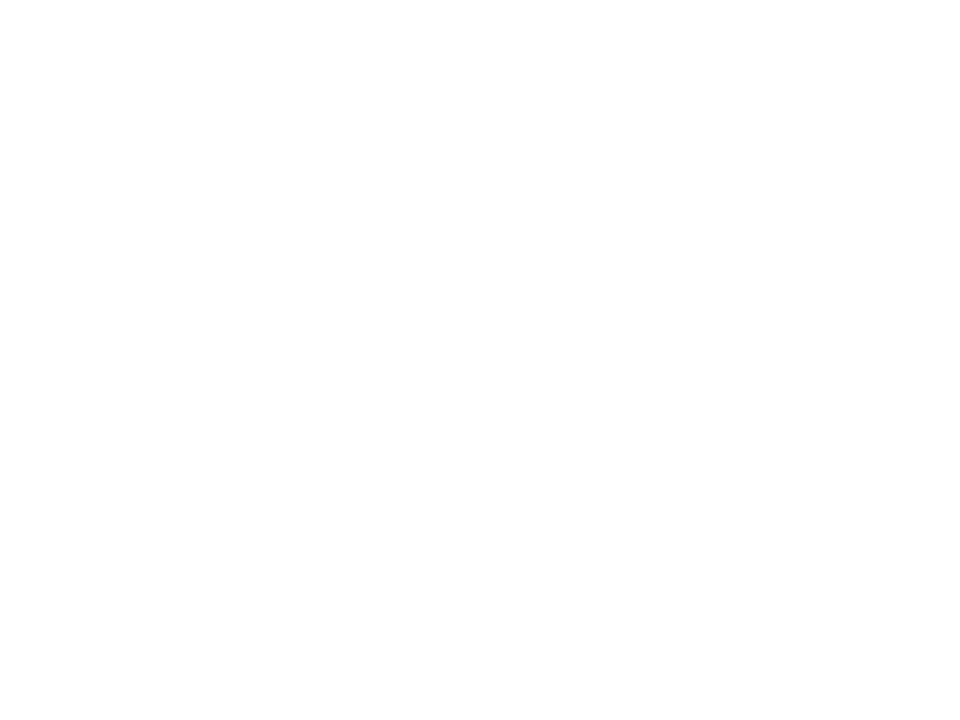
\includegraphics[width=0.8\textwidth]{plots/laufzeit.pdf}
    \caption{}
\end{figure}
Über die Ausgleichsgerade, nach
\begin{equation}
    t=m \cdot L+n,
\end{equation}
lässt sich nun der y-Achsenabschnitt $n$ bestimmen.
Er spiegelt einen systematischen Fehler wieder, der aus der Dicke der Anpassungsschicht
resultiert.\\ 
Für die Parameter ergibt sich
\begin{align*}
    m=0.37\frac{\mu s}{cm},\\
    n=0.33\mu s.
\end{align*}
Über die Laufzeitgeschwindigkeit $n$ und die Schallgeschwidigkeit von Wasser
$c_{\text{Wasser}}=343m/s$ der Anpassungsschicht kann nun mit
\begin{equation}
    d=\frac{1}{2} \cdot c_{\text{wasser}} \cdot n,
\end{equation}
die Dicke $d$ der Anpassungschicht mit
\begin{equation}
    d=0.56\mu m
\end{equation}
angegeben werden.
Für die angepasste Schallgeschwindikeit in Acyril ergibt sich somit nach
\begin{equation}
    c_{\text{echo,acyril}}=\frac{2L}{t-n}
\end{equation}
\begin{table}
    \centering
    \begin{tabular}{c| c c c}
        \toprule
        &Zylinder 1&Zylinder 2&Zylinder 3\\
        \midrule
        $c_{\text{echo,acyril}}$&&&\\
        \bottomrule
    \end{tabular}
    \caption{}
\end{table}


\subsection{Schallgeschwindigkeit (Durchschallungs-Verfahren)}
Über die gemessen Laufzeit $t$ kann die Schallgeschwindigkeit nach
\begin{equation}
    c_{\text{durch,acyril}}=\frac{2L}{t},
\end{equation}
berechnet werden.
Es ergibt sich
\begin{table}
    \centering
    \begin{tabular}{c| c c c}
        \toprule
        &Zylinder 1&Zylinder 2&Zylinder 3\\
        \midrule
        $c_{\text{durch,acyril}}$&&&\\
        \bottomrule
    \end{tabular}
    \caption{}
\end{table}

\subsection{Biometrische Untersuchung eines Augenmodells}

\label{sec:Auswertung}
